\section{栈的应用:表达式求值与转换}

\begin{figure}[H]
\centering
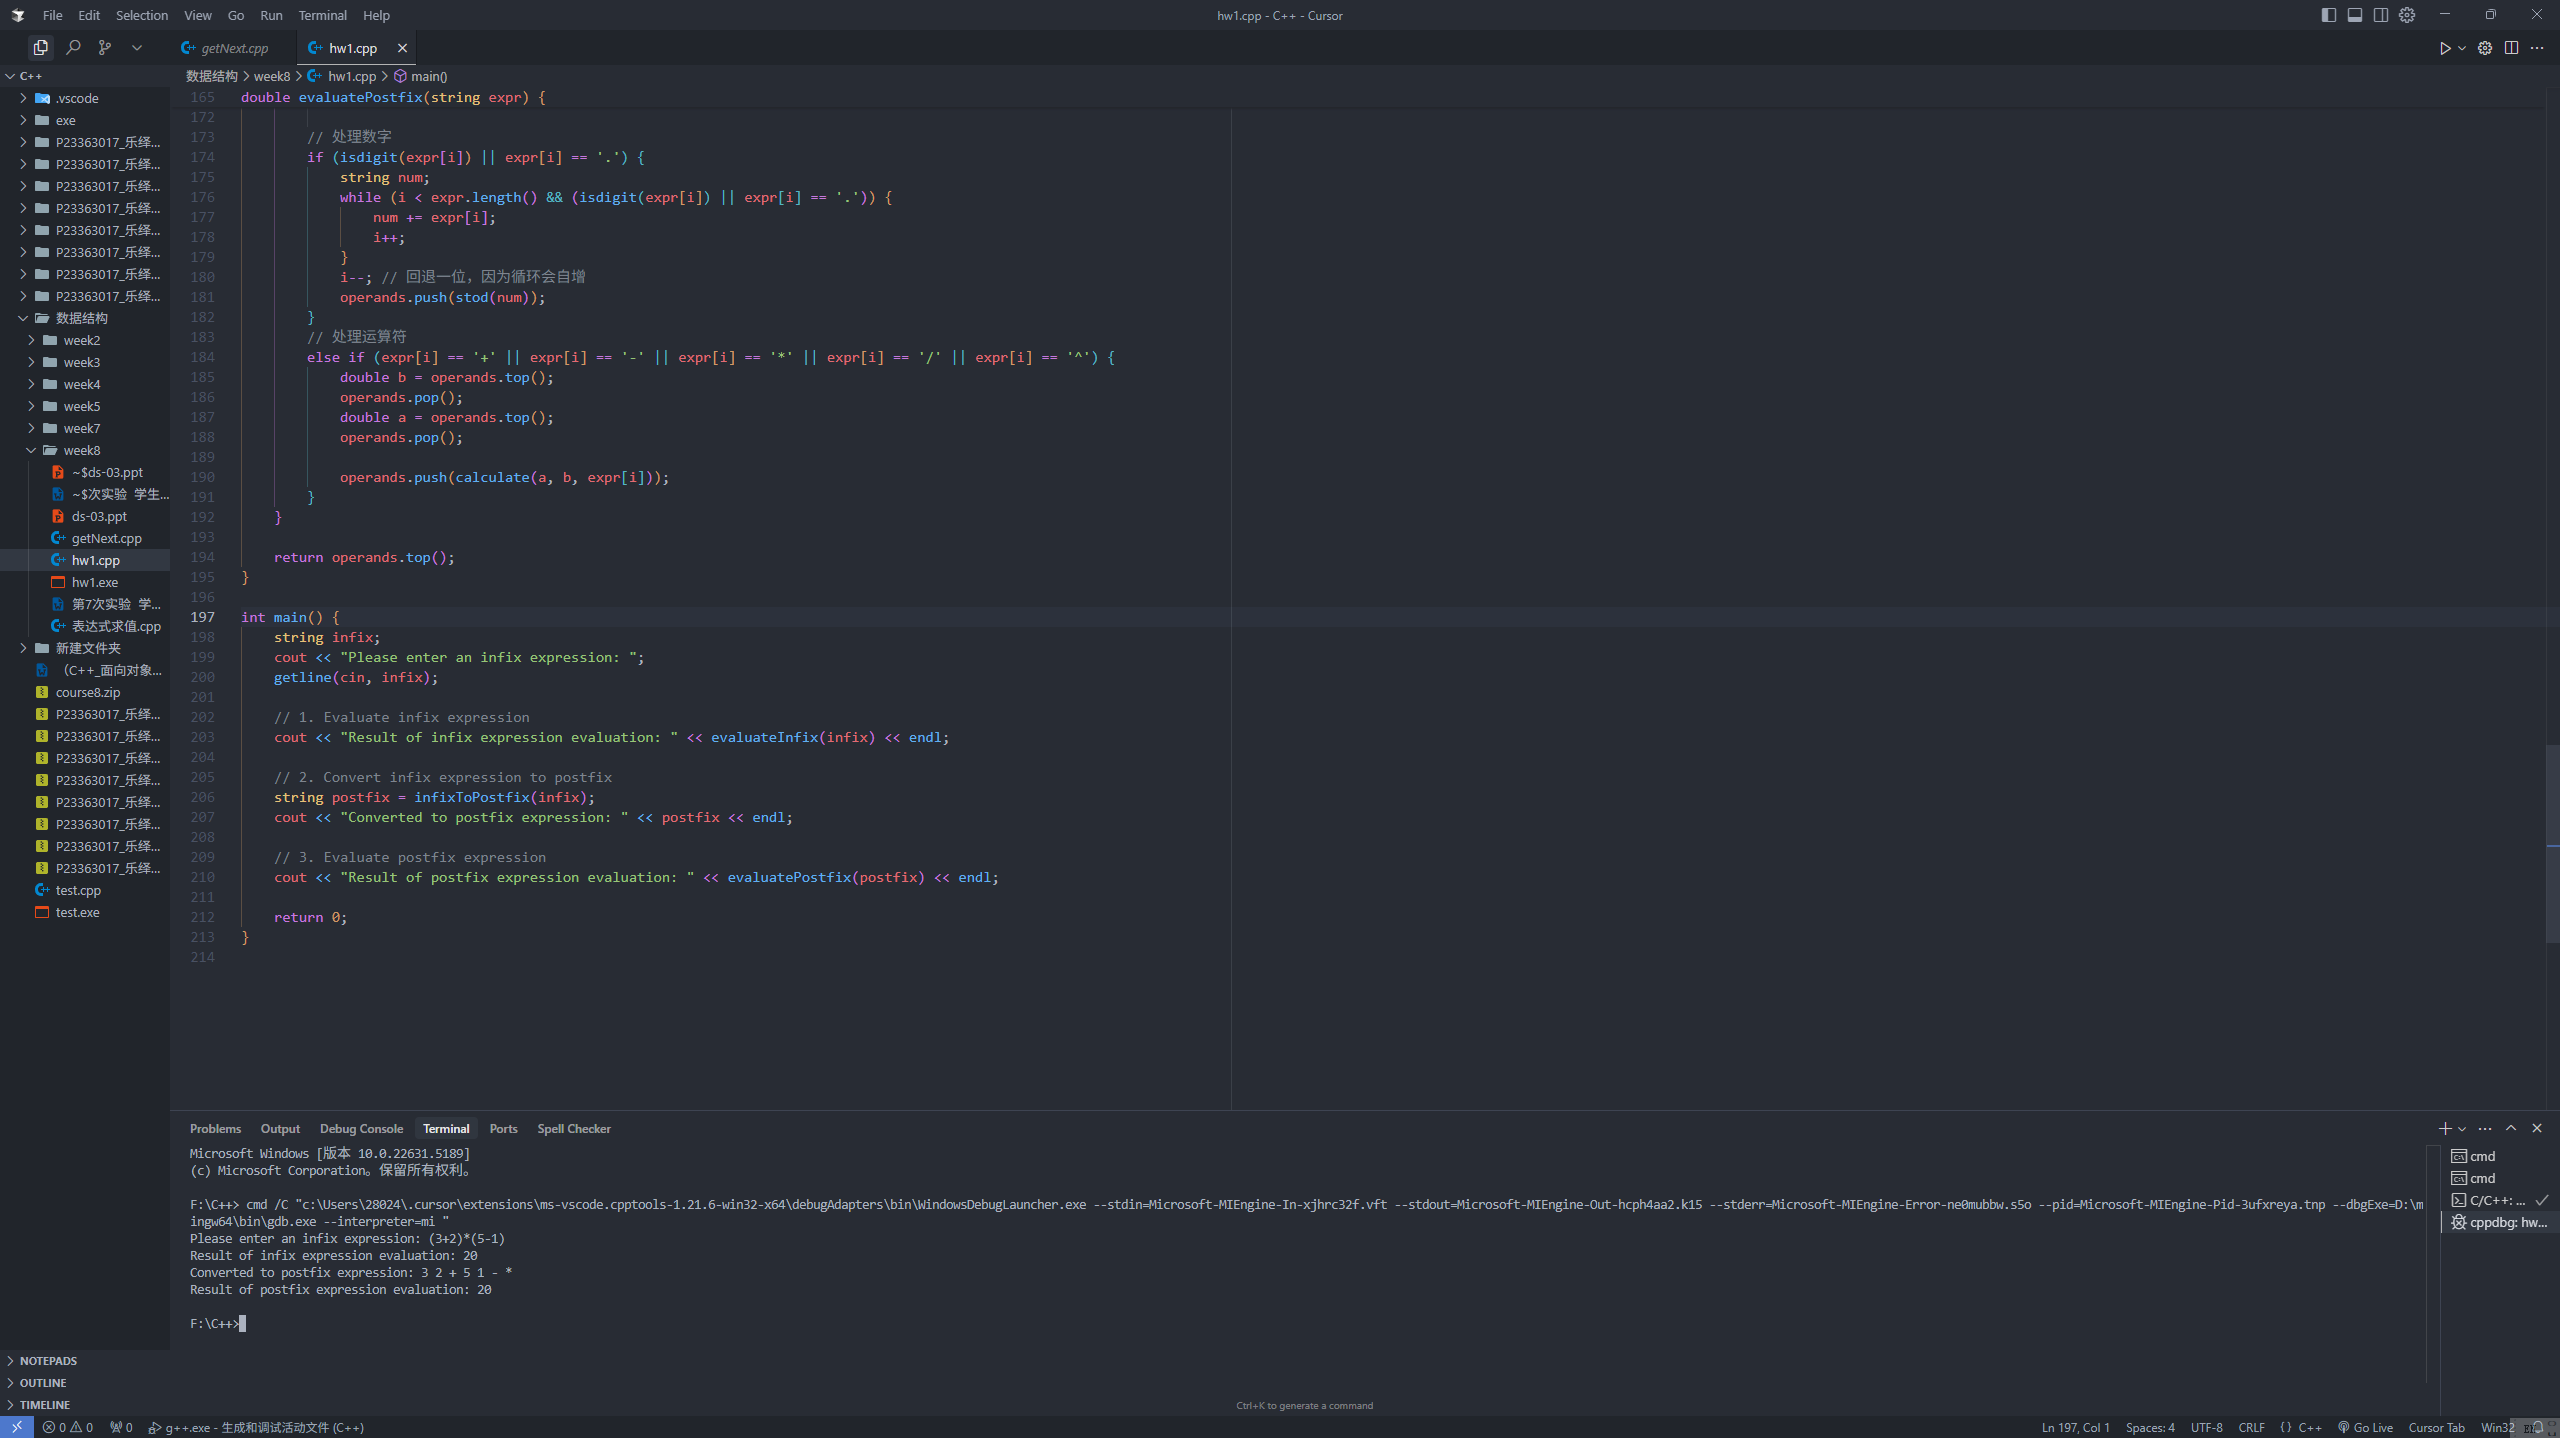
\includegraphics[width=\textwidth]{实验报告7-2025042122.png}
% \caption{}
\label{}
\end{figure}

\begin{lstlisting}[language=C++]
#include <iostream>

#include <stack>

#include <string>

#include <cctype>

#include <cmath>

using namespace std;

  

// 判断运算符优先级

int priority(char op) {

    if (op == '+' || op == '-')

        return 1;

    else if (op == '*' || op == '/')

        return 2;

    else if (op == '^')

        return 3;

    else

        return 0;

}

  

// 执行运算

double calculate(double a, double b, char op) {

    switch (op) {

        case '+': return a + b;

        case '-': return a - b;

        case '*': return a * b;

        case '/': return a / b;

        case '^': return pow(a, b);

        default: return 0;

    }

}

  

// 1. 中缀表达式求值

double evaluateInfix(string expr) {

    stack<double> operands;

    stack<char> operators;

    for (int i = 0; i < expr.length(); i++) {

        // 跳过空格

        if (expr[i] == ' ')

            continue;

        // 处理数字

        if (isdigit(expr[i]) || expr[i] == '.') {

            string num;

            while (i < expr.length() && (isdigit(expr[i]) || expr[i] == '.')) {

                num += expr[i];

                i++;

            }

            i--; // 回退一位,因为循环会自增

            operands.push(stod(num));

        }

        // 处理左括号

        else if (expr[i] == '(') {

            operators.push(expr[i]);

        }

        // 处理右括号

        else if (expr[i] == ')') {

            while (!operators.empty() && operators.top() != '(') {

                char op = operators.top();

                operators.pop();

                double b = operands.top();

                operands.pop();

                double a = operands.top();

                operands.pop();

                operands.push(calculate(a, b, op));

            }

            if (!operators.empty())

                operators.pop(); // 弹出左括号

        }

        // 处理运算符

        else if (expr[i] == '+' || expr[i] == '-' || expr[i] == '*' || expr[i] == '/' || expr[i] == '^') {

            while (!operators.empty() && operators.top() != '(' &&

                   priority(operators.top()) >= priority(expr[i])) {

                char op = operators.top();

                operators.pop();

                double b = operands.top();

                operands.pop();

                double a = operands.top();

                operands.pop();

                operands.push(calculate(a, b, op));

            }

            operators.push(expr[i]);

        }

    }

    // 处理剩余的运算符

    while (!operators.empty()) {

        char op = operators.top();

        operators.pop();

        double b = operands.top();

        operands.pop();

        double a = operands.top();

        operands.pop();

        operands.push(calculate(a, b, op));

    }

    return operands.top();

}

  

// 2. 中缀表达式转为后缀表达式

string infixToPostfix(string expr) {

    stack<char> operators;

    string postfix = "";

    for (int i = 0; i < expr.length(); i++) {

        // 跳过空格

        if (expr[i] == ' ')

            continue;

        // 处理数字

        if (isdigit(expr[i]) || expr[i] == '.') {

            string num;

            while (i < expr.length() && (isdigit(expr[i]) || expr[i] == '.')) {

                num += expr[i];

                i++;

            }

            i--; // 回退一位,因为循环会自增

            postfix += num + " ";

        }

        // 处理左括号

        else if (expr[i] == '(') {

            operators.push(expr[i]);

        }

        // 处理右括号

        else if (expr[i] == ')') {

            while (!operators.empty() && operators.top() != '(') {

                postfix += operators.top();

                postfix += " ";

                operators.pop();

            }

            if (!operators.empty())

                operators.pop(); // 弹出左括号

        }

        // 处理运算符

        else if (expr[i] == '+' || expr[i] == '-' || expr[i] == '*' || expr[i] == '/' || expr[i] == '^') {

            while (!operators.empty() && operators.top() != '(' &&

                   priority(operators.top()) >= priority(expr[i])) {

                postfix += operators.top();

                postfix += " ";

                operators.pop();

            }

            operators.push(expr[i]);

        }

    }

    // 处理剩余的运算符

    while (!operators.empty()) {

        postfix += operators.top();

        postfix += " ";

        operators.pop();

    }

    return postfix;

}

  

// 3. 后缀表达式求值

double evaluatePostfix(string expr) {

    stack<double> operands;

    for (int i = 0; i < expr.length(); i++) {

        // 跳过空格

        if (expr[i] == ' ')

            continue;

        // 处理数字

        if (isdigit(expr[i]) || expr[i] == '.') {

            string num;

            while (i < expr.length() && (isdigit(expr[i]) || expr[i] == '.')) {

                num += expr[i];

                i++;

            }

            i--; // 回退一位,因为循环会自增

            operands.push(stod(num));

        }

        // 处理运算符

        else if (expr[i] == '+' || expr[i] == '-' || expr[i] == '*' || expr[i] == '/' || expr[i] == '^') {

            double b = operands.top();

            operands.pop();

            double a = operands.top();

            operands.pop();

            operands.push(calculate(a, b, expr[i]));

        }

    }

    return operands.top();

}

  

int main() {

    string infix;

    cout << "Please enter an infix expression: ";

    getline(cin, infix);

    // 1. Evaluate infix expression

    cout << "Result of infix expression evaluation: " << evaluateInfix(infix) << endl;

    // 2. Convert infix expression to postfix

    string postfix = infixToPostfix(infix);

    cout << "Converted to postfix expression: " << postfix << endl;

    // 3. Evaluate postfix expression

    cout << "Result of postfix expression evaluation: " << evaluatePostfix(postfix) << endl;

    return 0;

}
\end{lstlisting}
\section{BF 算法查找}

\begin{figure}[H]
\centering
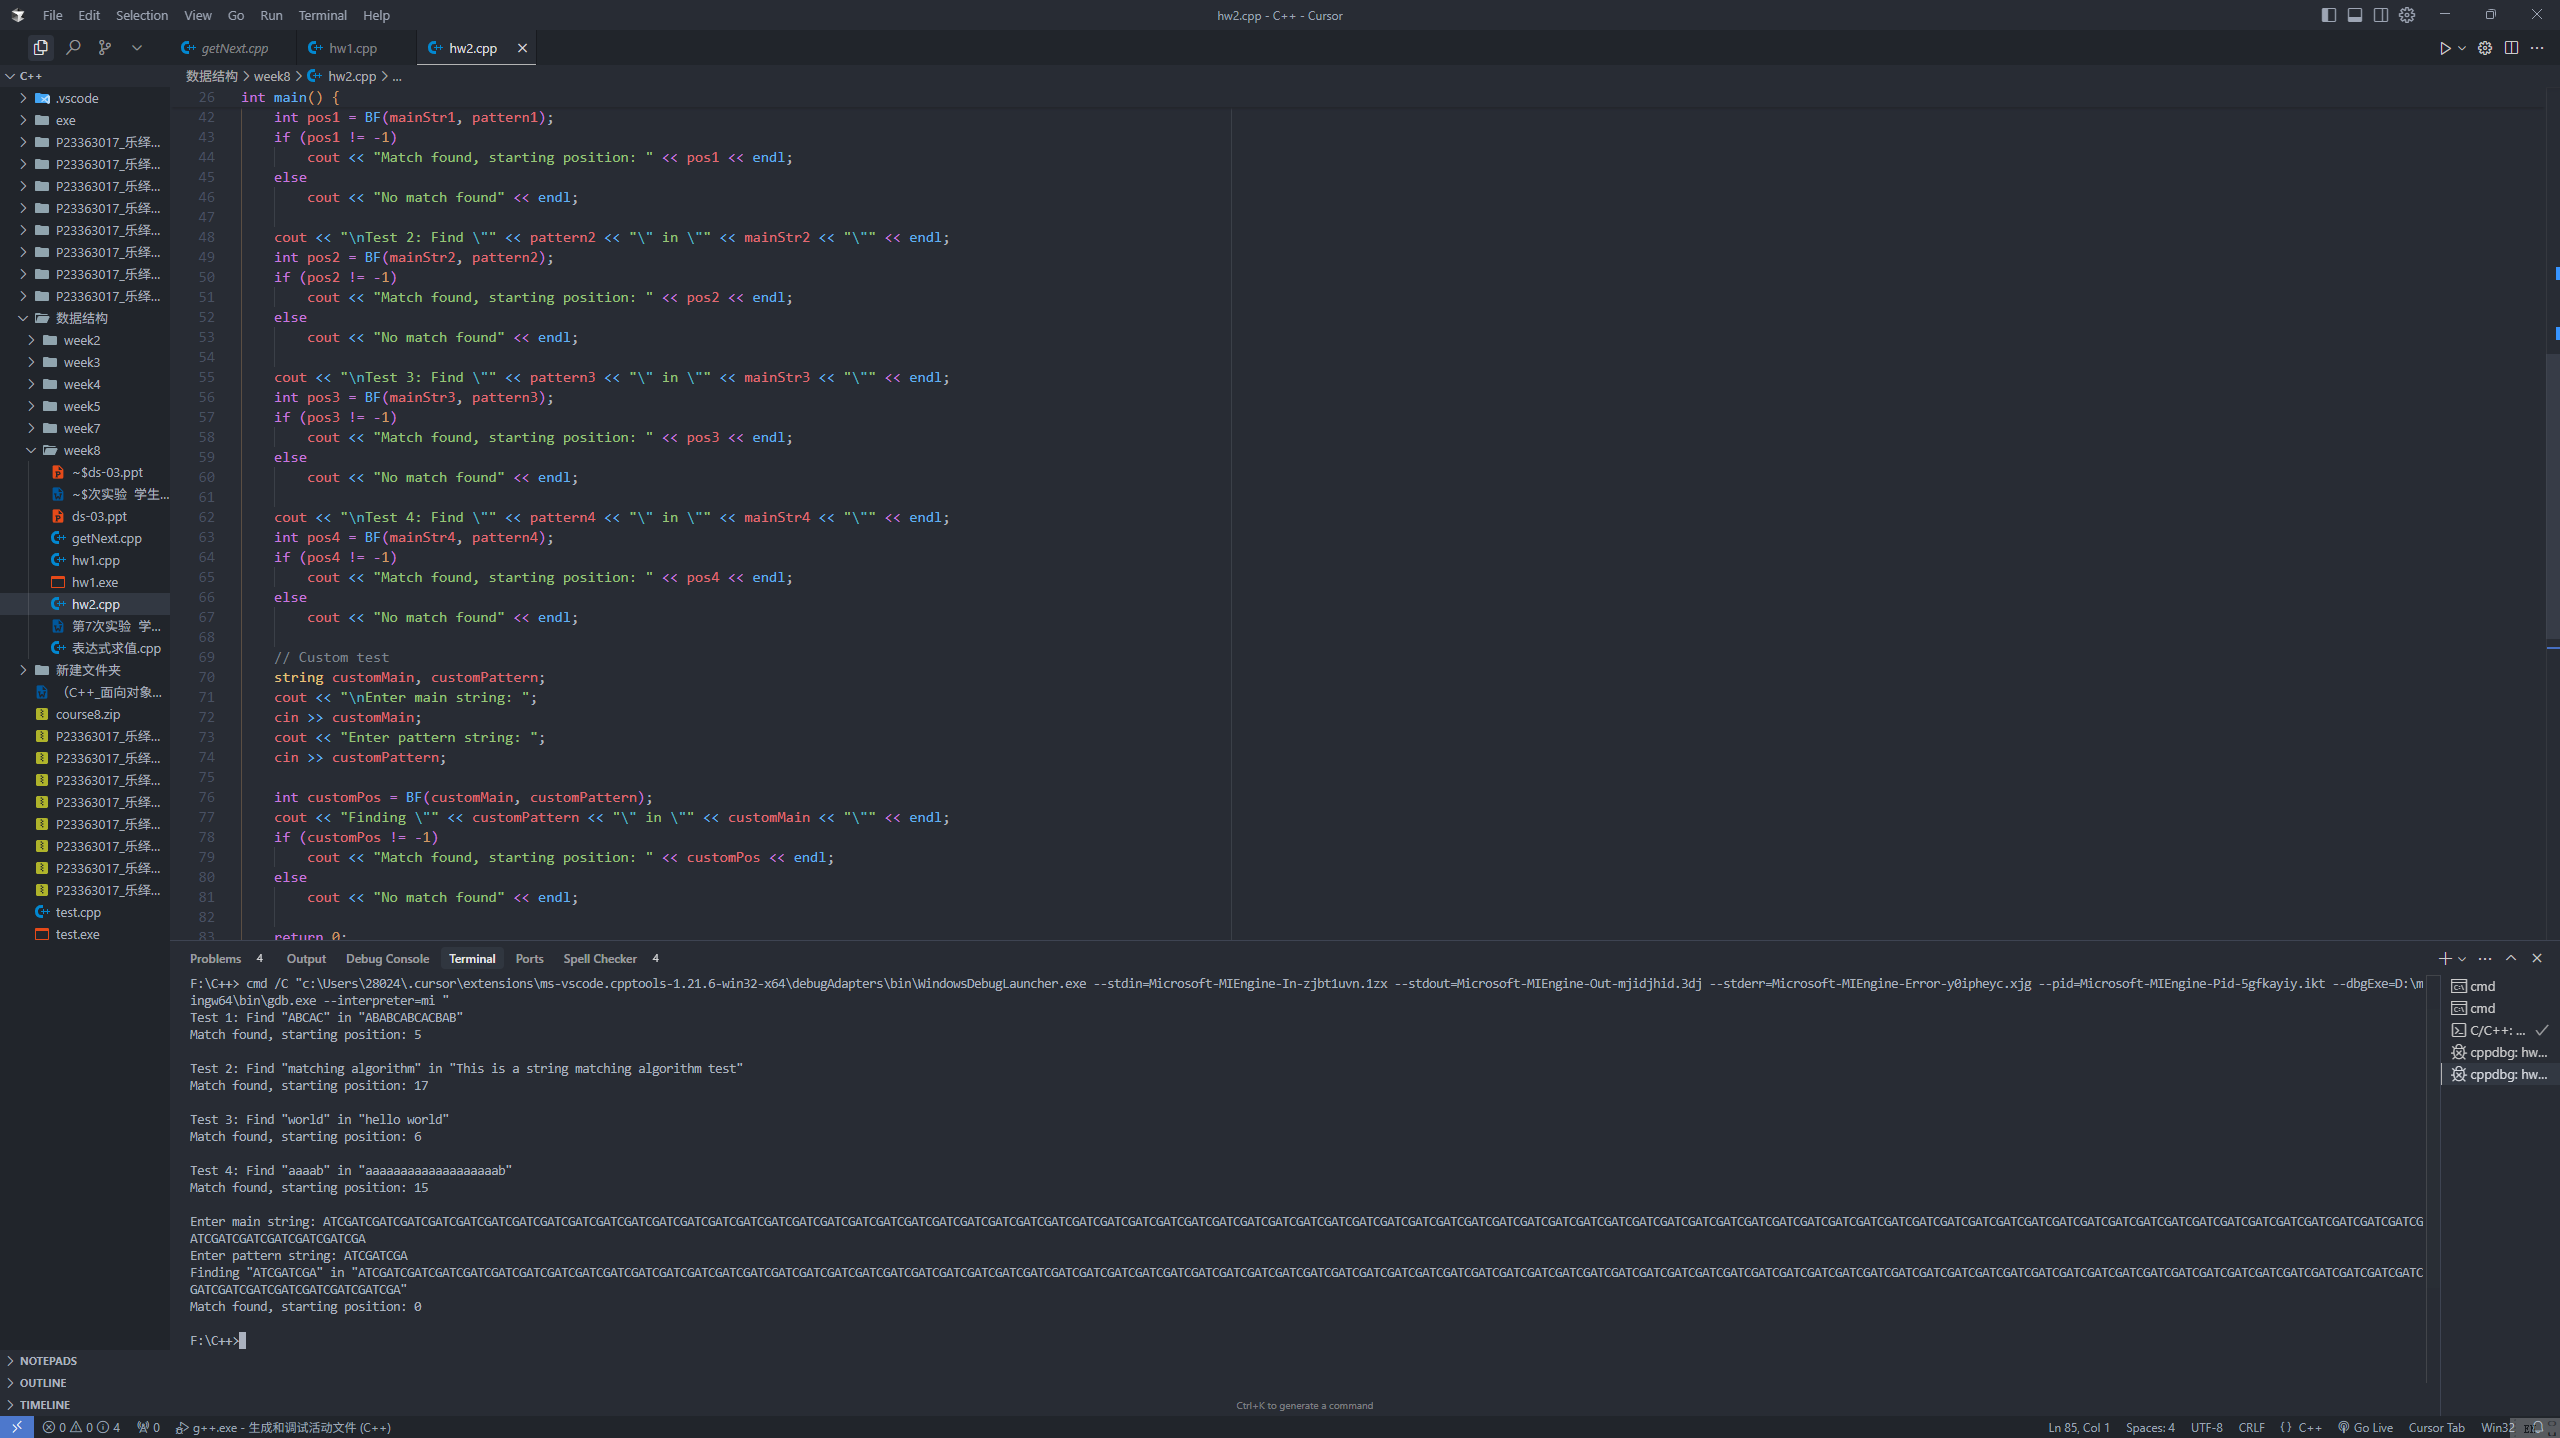
\includegraphics[width=\textwidth]{1-实验报告7-2025042122.png}
% \caption{}
\label{}
\end{figure}

\begin{lstlisting}[language=C++]
#include <iostream>

#include <string>

using namespace std;

  

// BF(Brute Force) algorithm implementation

int BF(const string& mainStr, const string& pattern) {

    int mainLen = mainStr.length();

    int patternLen = pattern.length();

    if (patternLen > mainLen) return -1;  // Pattern is longer than main string, no match possible

    for (int i = 0; i <= mainLen - patternLen; i++) {

        int j;

        for (j = 0; j < patternLen; j++) {

            if (mainStr[i + j] != pattern[j])

                break;  // Character mismatch, exit inner loop

        }

        if (j == patternLen)

            return i;  // Match found, return starting position

    }

    return -1;  // No match found

}

  

int main() {

    // Test cases

    string mainStr1 = "ABABCABCACBAB";

    string pattern1 = "ABCAC";

    string mainStr2 = "This is a string matching algorithm test";

    string pattern2 = "matching algorithm";

    string mainStr3 = "hello world";

    string pattern3 = "world";

    string mainStr4 = "aaaaaaaaaaaaaaaaaaab";

    string pattern4 = "aaaab";

    // Test and output results

    cout << "Test 1: Find \"" << pattern1 << "\" in \"" << mainStr1 << "\"" << endl;

    int pos1 = BF(mainStr1, pattern1);

    if (pos1 != -1)

        cout << "Match found, starting position: " << pos1 << endl;

    else

        cout << "No match found" << endl;

    cout << "\nTest 2: Find \"" << pattern2 << "\" in \"" << mainStr2 << "\"" << endl;

    int pos2 = BF(mainStr2, pattern2);

    if (pos2 != -1)

        cout << "Match found, starting position: " << pos2 << endl;

    else

        cout << "No match found" << endl;

    cout << "\nTest 3: Find \"" << pattern3 << "\" in \"" << mainStr3 << "\"" << endl;

    int pos3 = BF(mainStr3, pattern3);

    if (pos3 != -1)

        cout << "Match found, starting position: " << pos3 << endl;

    else

        cout << "No match found" << endl;

    cout << "\nTest 4: Find \"" << pattern4 << "\" in \"" << mainStr4 << "\"" << endl;

    int pos4 = BF(mainStr4, pattern4);

    if (pos4 != -1)

        cout << "Match found, starting position: " << pos4 << endl;

    else

        cout << "No match found" << endl;

    // Custom test

    string customMain, customPattern;

    cout << "\nEnter main string: ";

    cin >> customMain;

    cout << "Enter pattern string: ";

    cin >> customPattern;

    int customPos = BF(customMain, customPattern);

    cout << "Finding \"" << customPattern << "\" in \"" << customMain << "\"" << endl;

    if (customPos != -1)

        cout << "Match found, starting position: " << customPos << endl;

    else

        cout << "No match found" << endl;

    return 0;

}
\end{lstlisting}
\section{KMP 算法查找位置}

\begin{figure}[H]
\centering
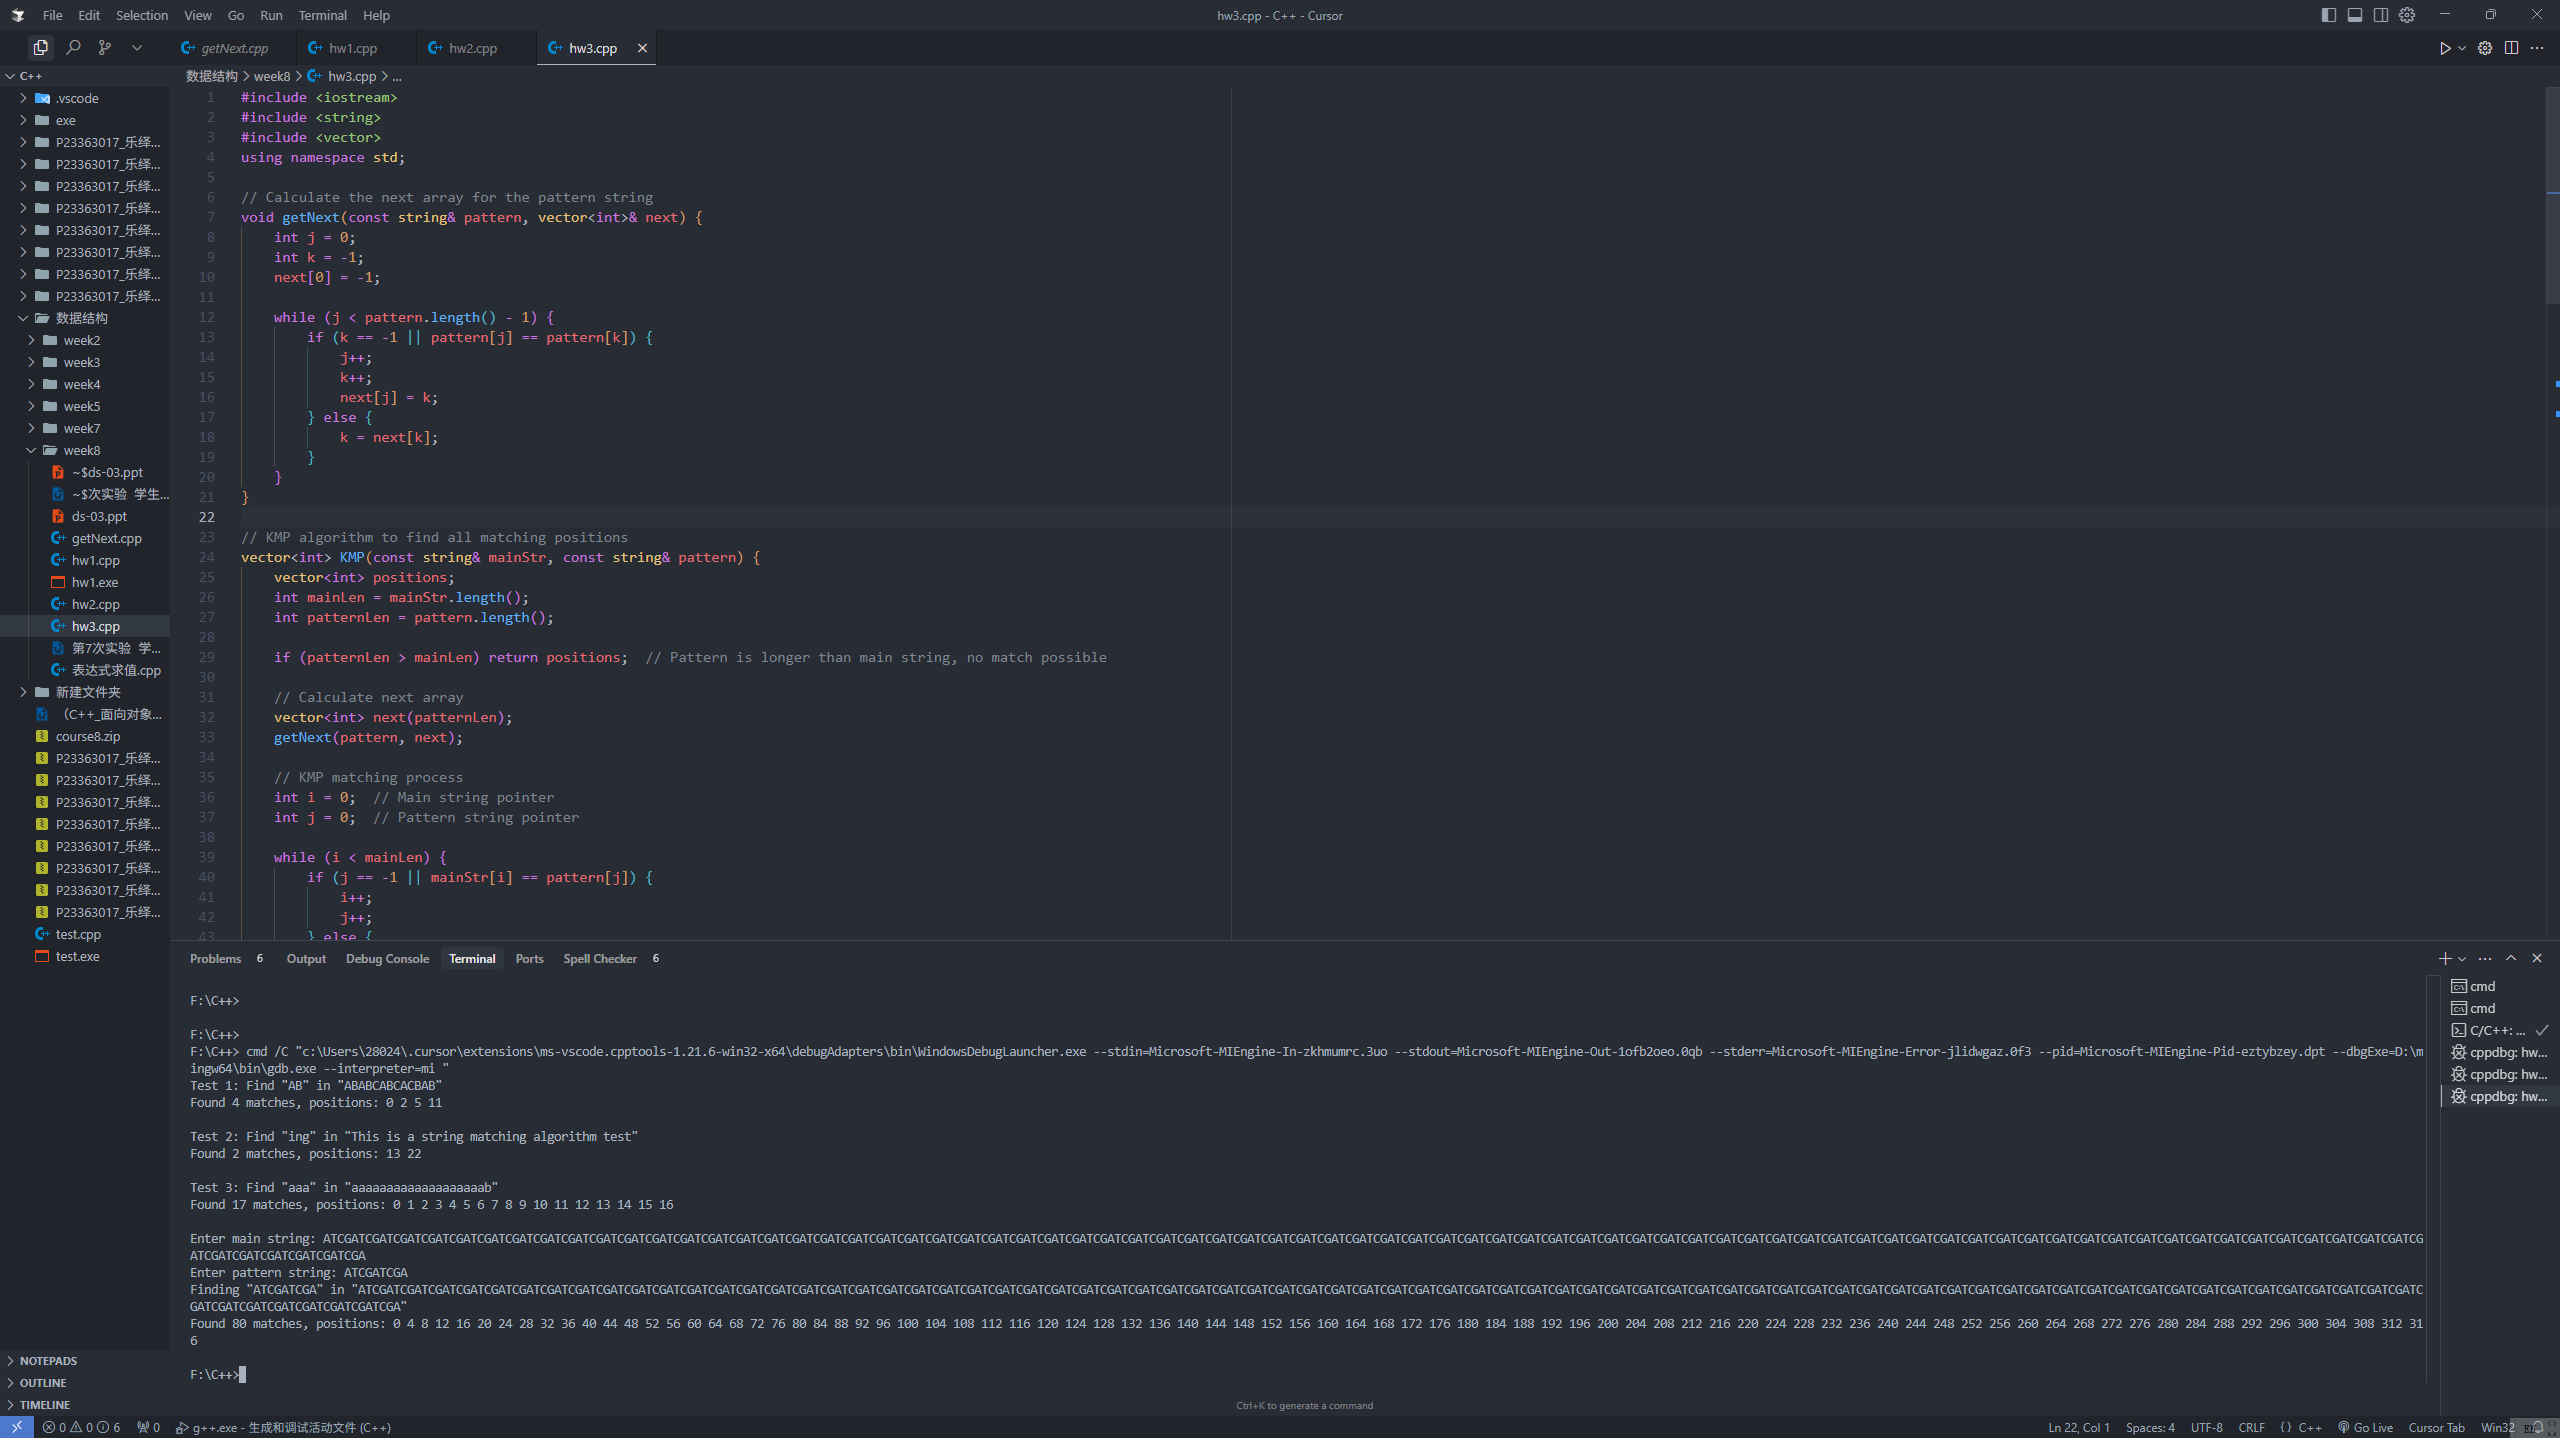
\includegraphics[width=\textwidth]{3-实验报告7-2025042122.png}
% \caption{}
\label{}
\end{figure}

\begin{lstlisting}[language=C++]
#include <iostream>

#include <string>

#include <vector>

using namespace std;

  

// Calculate the next array for the pattern string

void getNext(const string& pattern, vector<int>& next) {

    int j = 0;

    int k = -1;

    next[0] = -1;

    while (j < pattern.length() - 1) {

        if (k == -1 || pattern[j] == pattern[k]) {

            j++;

            k++;

            next[j] = k;

        } else {

            k = next[k];

        }

    }

}

  

// KMP algorithm to find all matching positions

vector<int> KMP(const string& mainStr, const string& pattern) {

    vector<int> positions;

    int mainLen = mainStr.length();

    int patternLen = pattern.length();

    if (patternLen > mainLen) return positions;  // Pattern is longer than main string, no match possible

    // Calculate next array

    vector<int> next(patternLen);

    getNext(pattern, next);

    // KMP matching process

    int i = 0;  // Main string pointer

    int j = 0;  // Pattern string pointer

    while (i < mainLen) {

        if (j == -1 || mainStr[i] == pattern[j]) {

            i++;

            j++;

        } else {

            j = next[j];

        }

        if (j == patternLen) {  // Found a match

            positions.push_back(i - j);  // Record the starting position of the match

            j = next[j-1];  // Continue to find the next match

            i--;  // Go back one position, as i was already incremented

        }

    }

    return positions;

}

  

int main() {

    // Test cases

    string mainStr1 = "ABABCABCACBAB";

    string pattern1 = "AB";

    string mainStr2 = "This is a string matching algorithm test";

    string pattern2 = "ing";

    string mainStr3 = "aaaaaaaaaaaaaaaaaaab";

    string pattern3 = "aaa";

    // Test and output results

    cout << "Test 1: Find \"" << pattern1 << "\" in \"" << mainStr1 << "\"" << endl;

    vector<int> pos1 = KMP(mainStr1, pattern1);

    if (!pos1.empty()) {

        cout << "Found " << pos1.size() << " matches, positions: ";

        for (int p : pos1) {

            cout << p << " ";

        }

        cout << endl;

    } else {

        cout << "No match found" << endl;

    }

    cout << "\nTest 2: Find \"" << pattern2 << "\" in \"" << mainStr2 << "\"" << endl;

    vector<int> pos2 = KMP(mainStr2, pattern2);

    if (!pos2.empty()) {

        cout << "Found " << pos2.size() << " matches, positions: ";

        for (int p : pos2) {

            cout << p << " ";

        }

        cout << endl;

    } else {

        cout << "No match found" << endl;

    }

    cout << "\nTest 3: Find \"" << pattern3 << "\" in \"" << mainStr3 << "\"" << endl;

    vector<int> pos3 = KMP(mainStr3, pattern3);

    if (!pos3.empty()) {

        cout << "Found " << pos3.size() << " matches, positions: ";

        for (int p : pos3) {

            cout << p << " ";

        }

        cout << endl;

    } else {

        cout << "No match found" << endl;

    }

    // Custom test

    string customMain, customPattern;

    cout << "\nEnter main string: ";

    cin >> customMain;

    cout << "Enter pattern string: ";

    cin >> customPattern;

    vector<int> customPos = KMP(customMain, customPattern);

    cout << "Finding \"" << customPattern << "\" in \"" << customMain << "\"" << endl;

    if (!customPos.empty()) {

        cout << "Found " << customPos.size() << " matches, positions: ";

        for (int p : customPos) {

            cout << p << " ";

        }

        cout << endl;

    } else {

        cout << "No match found" << endl;

    }

    return 0;

}
\end{lstlisting}
\section{队列的应用}

\begin{figure}[H]
\centering
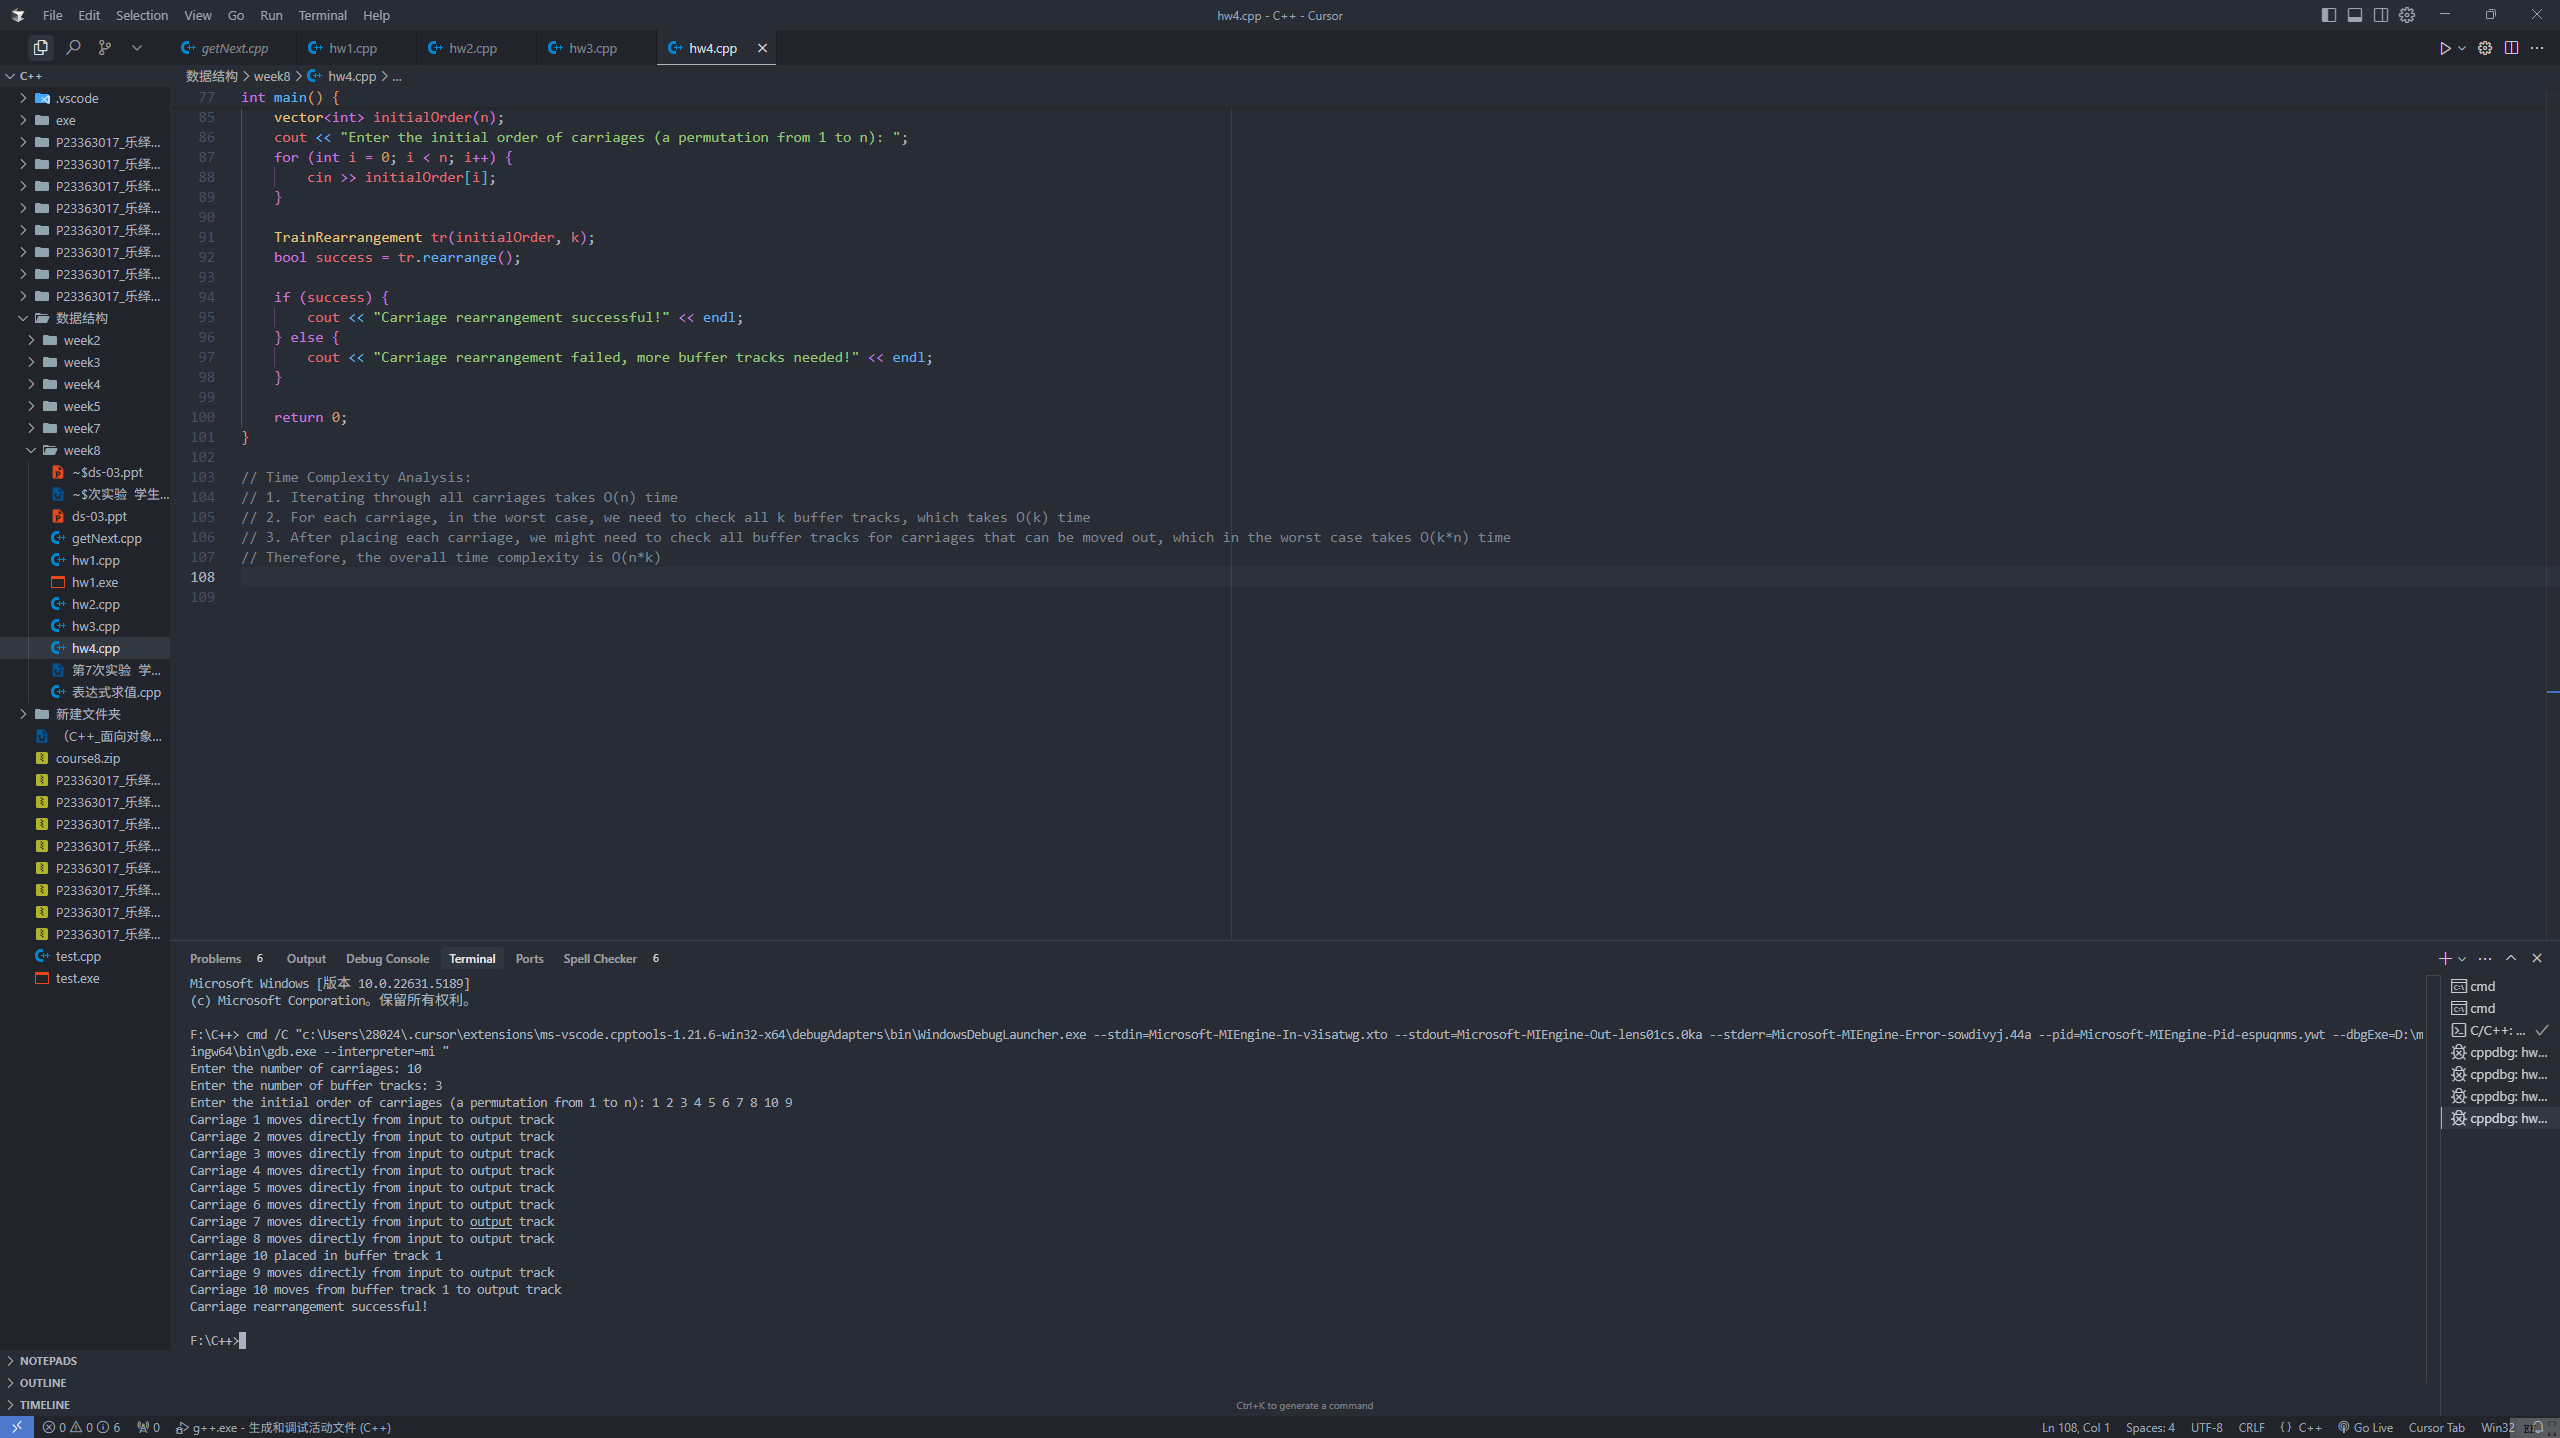
\includegraphics[width=\textwidth]{4-实验报告7-2025042122.png}
% \caption{}
\label{}
\end{figure}

\begin{lstlisting}[language=C++]
#include <iostream>

#include <queue>

#include <stack>

#include <vector>

using namespace std;

  

// Train Rearrangement Problem

class TrainRearrangement {

private:

    vector<int> initialOrder;    // Initial order of carriages

    int n;                       // Number of carriages

    int k;                       // Number of buffer tracks

    vector<queue<int>> bufferTracks; // K buffer tracks

  

public:

    TrainRearrangement(vector<int>& order, int bufferNum) {

        initialOrder = order;

        n = order.size();

        k = bufferNum;

        bufferTracks.resize(k);

    }

  

    // Rearrange carriages

    bool rearrange() {

        // Target is to arrange carriages in order from 1 to n

        int nextNeeded = 1;

        // Simulate the input track operation

        for (int i = 0; i < n; i++) {

            int current = initialOrder[i];

            // If the current carriage is the one we need, send it directly to the output track

            if (current == nextNeeded) {

                cout << "Carriage " << current << " moves directly from input to output track" << endl;

                nextNeeded++;

                // Check if there are any carriages in buffer tracks that can be moved out

                bool foundInBuffer = true;

                while (foundInBuffer) {

                    foundInBuffer = false;

                    for (int j = 0; j < k; j++) {

                        if (!bufferTracks[j].empty() && bufferTracks[j].front() == nextNeeded) {

                            cout << "Carriage " << nextNeeded << " moves from buffer track " << j+1 << " to output track" << endl;

                            bufferTracks[j].pop();

                            nextNeeded++;

                            foundInBuffer = true;

                            break;

                        }

                    }

                }

            } else {

                // Need to place the carriage in a buffer track

                bool placed = false;

                for (int j = 0; j < k; j++) {

                    // Try to find an empty buffer track or one where the top carriage number is greater than the current one

                    if (bufferTracks[j].empty() || bufferTracks[j].back() > current) {

                        bufferTracks[j].push(current);

                        cout << "Carriage " << current << " placed in buffer track " << j+1 << endl;

                        placed = true;

                        break;

                    }

                }

                // If it cannot be placed in any buffer track, rearrangement fails

                if (!placed) {

                    cout << "Cannot rearrange carriages: insufficient buffer tracks" << endl;

                    return false;

                }

            }

        }

        // Check if all carriages have been arranged in order

        return nextNeeded > n;

    }

};

  

int main() {

    int n, k;

    cout << "Enter the number of carriages: ";

    cin >> n;

    cout << "Enter the number of buffer tracks: ";

    cin >> k;

    vector<int> initialOrder(n);

    cout << "Enter the initial order of carriages (a permutation from 1 to n): ";

    for (int i = 0; i < n; i++) {

        cin >> initialOrder[i];

    }

    TrainRearrangement tr(initialOrder, k);

    bool success = tr.rearrange();

    if (success) {

        cout << "Carriage rearrangement successful!" << endl;

    } else {

        cout << "Carriage rearrangement failed, more buffer tracks needed!" << endl;

    }

    return 0;

}

  

// Time Complexity Analysis:

// 1. Iterating through all carriages takes O(n) time

// 2. For each carriage, in the worst case, we need to check all k buffer tracks, which takes O(k) time

// 3. After placing each carriage, we might need to check all buffer tracks for carriages that can be moved out, which in the worst case takes O(k*n) time

// Therefore, the overall time complexity is O(n*k)
\end{lstlisting}